        \clearpage
        \begin{figure*}[ht]
            \pdfbookmark[2]{ID 02}{figure_id_02}
        	\centering
            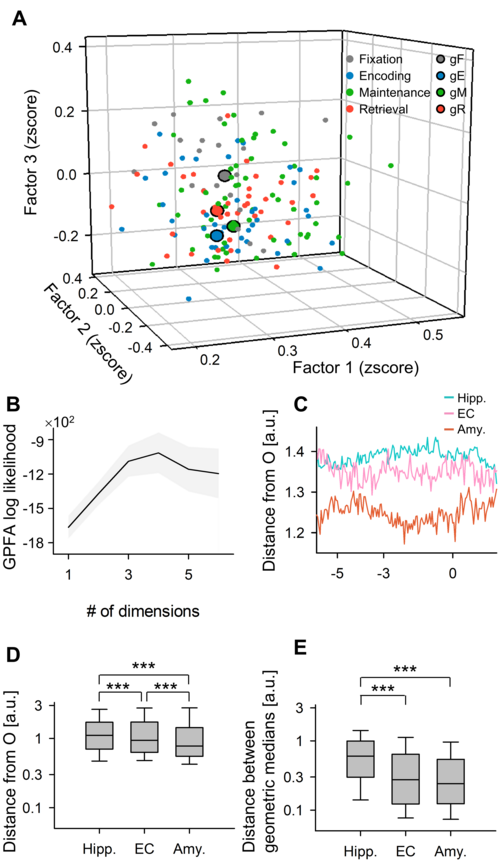
\includegraphics[width=0.5\textwidth]{./media/figures/.png/Figure_ID_02.png}
        	\caption{\textbf{
State-dependent hippocampal neural trajectory
}
\smallskip
\\
\textbf{\textit{A.}} Neural Trajectory Visualization: This three-dimensional plot represents the neural trajectory of the left hippocampus derived from the Gaussian-process factor analysis (GPFA). Smaller points indicate coordinates of 50-ms neural trajectory bins within a session (median of 50 trials). Larger points with \textit{black} edges represent geometric medians for each phase of the Sternberg working memory task, distinguished by colors for fixation (\textit{gray}), encoding (\textit{blue}), maintenance (\textit{green}), and retrieval (\textit{red}). \textbf{\textit{B.}}  GPFA Model Log-likelihoods: The graph showcases the log-likelihood predictions of GPFA models concerning the number of dimensions. Notably, the optimal dimension was identified as three using the elbow method. \textbf{\textit{C.}}  Distance Analysis from $O$rigin: The plot represents the trajectory distance from the origin ($O$) for the hippocampus (Hipp.), entorhinal cortex (EC), and amygdala (Amy.), plotted against the time since probe onset. \textbf{\textit{D.}}  Trajectory Distance in Medial Temporal Regions: The box plots display the trajectory distances from $O$ for each region, with the hippocampus showing the greatest distance, followed by the EC and the Amygdala. \textbf{\textit{E.}}  Inter-phase Trajectory Distances: This visualizes the distance variations between trial trajectory geometric medians of task phases. The distances in the hippocampus were observed to be more pronounced compared to the EC or Amygdala.
}
% width=0.5\textwidth
        	\label{fig:02}
        \end{figure*}
